\documentclass[a4paper,12pt]{article}

%%% Работа с русским языком
\usepackage{cmap}					% поиск в PDF
\usepackage{mathtext} 				% русские буквы в формулах
\usepackage[T2A]{fontenc}			% кодировка
\usepackage[utf8]{inputenc}			% кодировка исходного текста
\usepackage[english,russian]{babel}	% локализация и переносы

%%% Дополнительная работа с математикой
\usepackage{amsmath,amsfonts,amssymb,amsthm,mathtools} % AMS
\usepackage{icomma} % "Умная" запятая: $0,2$ --- число, $0, 2$ --- перечисление

%% Номера формул
%\mathtoolsset{showonlyrefs=true} % Показывать номера только у тех формул, на которые есть \eqref{} в тексте.
%\usepackage{leqno} % Нумерация формул слева

%% Свои команды
\DeclareMathOperator{\sgn}{\mathop{sgn}}

%% Перенос знаков в формулах (по Львовскому)
\newcommand*{\hm}[1]{#1\nobreak\discretionary{}
{\hbox{$\mathsurround=0pt #1$}}{}}

%%% Работа с картинками
\usepackage{graphicx}  % Для вставки рисунков
\graphicspath{{materials}{images2/}}  % папки с картинками
\setlength\fboxsep{3pt} % Отступ рамки \fbox{} от рисунка
\setlength\fboxrule{1pt} % Толщина линий рамки \fbox{}
\usepackage{wrapfig} % Обтекание рисунков текстом

%%% Работа с таблицами
\usepackage{array,tabularx,tabulary,booktabs} % Дополнительная работа с таблицами
\usepackage{longtable}  % Длинные таблицы
\usepackage{multirow} % Слияние строк в таблице

%%% Теоремы
\theoremstyle{plain} % Это стиль по умолчанию, его можно не переопределять.
\newtheorem{theorem}{Теорема}[section]
\newtheorem{proposition}[theorem]{Утверждение}
 
\theoremstyle{definition} % "Определение"
\newtheorem{corollary}{Следствие}[theorem]
\newtheorem{problem}{Задача}[section]
 
\theoremstyle{remark} % "Примечание"
\newtheorem*{nonum}{Решение}

%%% Программирование
\usepackage{etoolbox} % логические операторы

%%% Страница
%\usepackage{extsizes} % Возможность сделать 14-й шрифт
\usepackage{geometry} % Простой способ задавать поля
	\geometry{top=25mm}
	\geometry{bottom=30mm}
	\geometry{left=25mm}
	\geometry{right=25mm}
 %

%%% Способ сделать тоже самое(но красивее:)
%\usepackage[margin=0.8in]{geometry}

 
\usepackage{fancyhdr} % Колонтитулы
 	\pagestyle{fancy}
 	\renewcommand{\headrulewidth}{0mm}  % Толщина линейки, отчеркивающей верхний колонтитул
 	\lfoot{}
 	\rfoot{}
 	\rhead{}
 	\chead{}
 	\lhead{ }
 	% \cfoot{Нижний в центре} % По умолчанию здесь номер страницы

\usepackage{setspace} % Интерлиньяж
%\onehalfspacing % Интерлиньяж 1.5
%\doublespacing % Интерлиньяж 2
%\singlespacing % Интерлиньяж 1

\usepackage{lastpage} % Узнать, сколько всего страниц в документе.

\usepackage{soulutf8} % Модификаторы начертания

\usepackage{hyperref}
\usepackage[usenames,dvipsnames,svgnames,table,rgb]{xcolor}
\hypersetup{				% Гиперссылки
    unicode=true,           % русские буквы в раздела PDF
    pdftitle={Заголовок},   % Заголовок
    pdfauthor={Автор},      % Автор
    pdfsubject={Тема},      % Тема
    pdfcreator={Создатель}, % Создатель
    pdfproducer={Производитель}, % Производитель
    pdfkeywords={keyword1} {key2} {key3}, % Ключевые слова
    colorlinks=true,       	% false: ссылки в рамках; true: цветные ссылки
    linkcolor=red,          % внутренние ссылки
    citecolor=green,        % на библиографию
    filecolor=magenta,      % на файлы
    urlcolor=blue           % на URL
}

%\renewcommand{\familydefault}{\sfdefault} % Начертание шрифта

\usepackage{multicol} % Несколько колонок

% Мои "дополнительные" пакеты
\usepackage{textcase} 
\usepackage{pdfpages}
\usepackage{amsmath}
\usepackage{titlesec}
\usepackage{floatrow}

\usepackage{subfig}

\author{Подкидышев Алексей}
\title{Студент МФТИ ФИВТ - 3ый курс}
\date{\today}

%% Делаем красивый header:
\fancyhead[RO]{\footnotesize{\scshape\nouppercase{~\leftmark}}}
%% Делаем красивый header END

%Делаем большой отступ между section и subsection
\titlespacing*{\section} {0pt}{3.5ex plus 1ex minus .2ex}{2.7ex plus .2ex}
\titlespacing*{\subsection} {0pt}{2.7ex plus 1ex minus .2ex}{1ex plus .2ex}


\begin{document} % конец преамбулы, начало документа

\begin{center}
	\textit{\MakeTextUppercase{федеральное государственное автономное учреждение}}
		
	\vspace{0.5ex}
	
	\textbf{ \\ \MakeTextUppercase{<<Московский Физико-технический институт>>}}
\end{center}
\vspace{13ex}
\begin{flushright}
    \noindent
	{Подкидышев Алексей}
	\\
	\textit{Студент факультета инноваций\\ и высоких технологий\\(группа 792)}
\end{flushright}
\begin{center}
	\vspace{23ex}
	\line(1,0){430}\\[4ex]
	{\LARGE\textbf{Лабораторная работа 5.1}}
	\vspace{2ex}\\
	\textbf{\large{<<Измерение коэффициента ослабления $\gamma$-лучей в веществе и определение их энергии>>}}\\[3ex]
	\line(1,0){430}\\[5ex]
	\vfill
	Долгопрудный 
	
	{\today}
\end{center}

\newpage
\newpage
\renewcommand{\headrulewidth}{1pt}

\section{Описание работы}

\subsection{Теория}

Ослабление гамма-излучения в веществе:
\[I = I_0e^{-\mu l} (I = I_0e^{-\mu'm_1 l}),\]
где $I, I_0$ - интенсивности прошедшего и падающего излучений, $l$ - длина пути, пройденного пучком гамма-лучей, $m_1$ - масса пройденного вещества, приходящаяся на единицу площади. Константа $\mu'$, в отличие от $\mu$, не зависит от плотности среды.\par
Отсюда получим, что 
\[\mu = \frac{1}{l} \ln{\frac{N_0}{N}}.\]
Ослабление потока гамма-лучей связано с тремя эффектами: фотоэлектрическим поглощением, комптоновским рассеянием и с генерацией электрон-позитронных пар.\par
Фотоэлектрическое поглощение -- поглощение гамма-квантов при их столкновении с электронами внутренних атомных оболочек.
\[\mu_f = \sigma_f n_1,\]
где $n_1$ -- плотность внутренних электронов, $\sigma_f$ -- поперечное сечение фотоэлектрического поглощения.
\begin{figure}[h]
    \centering
    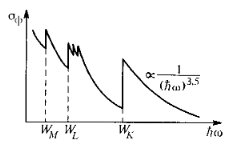
\includegraphics{img1.png}
    \caption{Зависимость сечения фотоэффекта от энергии гамма-квантов}
    \label{fig:my_label}
\end{figure}
Как видно из графика (рис. 1), фотоэффект является доминирующим механизмом поглощения при не очень высоких энергиях.\par
Комптоновское рассеяние -- рассеяние гамма-квантов на свободных (слабосвязанных) электронах. Роль эффекта Комптона становится заметной, когда энергия квантов становится много больше энергии связи электронов в атоме.
\[\sigma_k = \pi r \frac{mc^2}{\overline{h}\omega}\left(\ln{\frac{2\overline{h}\omega}{mc^2}} + \frac{1}{2}\right).\]
Образование пар происходит при энергиях гамма-лучей больше $2mc^2 = 1.02$ МэВ. При таких энергиях вероятность фотоэффекта не играет никакой роли и вероятность рождения пар сравнивается с вероятностью комптоновского рассеяния. Для свинца это энергии около $4.7$ эВ.\par
\newpage
Полный линейный коэффициент ослабления образуется из суммы трех коэффициентов.
\begin{figure}[h]
    \centering
    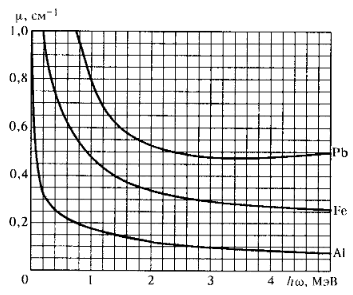
\includegraphics[width=0.5 \textwidth]{img2.png}
    \caption{Полные коэффициенты ослабления потока гамма-лучей в алюминии, железе и свинце}
    \label{fig:my_label}
\end{figure}
\begin{figure}[h]
    \centering
    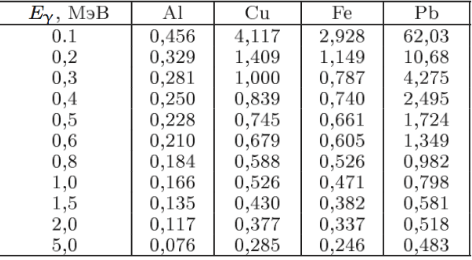
\includegraphics[width=0.5 \textwidth]{img3.png}
    \caption{Коэффициенты ослабления гамма квантов в различных веществах в зависимости от их энергии}
    \label{fig:my_label}
\end{figure}

\subsection{Экспериментальная установка}

Свинцовый коллиматор выпускает пучок почти параллельных гамма-квантов, который проходит через набор поглотителей П и регистрируется счетчиком. Сигналы от счетчика усиливаются и попадают в пересчетный прибор ПП. Высоковольтный выпрямитель ВВ обеспечивает работу сцинтилляционного счетчика. В результатах опыта могут наблюдаться высокие погрешности, это может быть связано с плохой геометрией опыта. 
\begin{figure}[h]
    \centering
    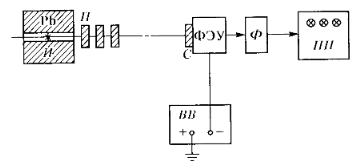
\includegraphics[width=0.5 \textwidth]{img4.png}
    \caption{Блок-схема установки}
    \label{fig:my_label}
\end{figure}
\newpage
Гамма-квант может несколько раз провзаимодействовать до того, как попадет на детектор (пути таких квантов показаны на рис. 5). Чтобы избежать этого, в нашей установке поглотители имеют небольшой размер, а счетчик расположен на достаточном большом расстоянии. 
\begin{figure}[h]
    \centering
    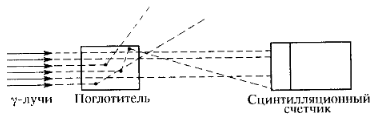
\includegraphics[width=0.5 \textwidth]{img5.png}
    \caption{Схема рассеяния гамма-квантов в поглотителе}
    \label{fig:my_label}
\end{figure}

\section{Ход работы}

\begin{enumerate}
    \item Будем проводить все измерения в течение $10$ с. Для начала измерим фон, обусловленный шумом ФЭУ и посторонними частицами, для этого закроем коллиматор толстой свинцовой пробкой:
    \[N_f = 672.\]
    Проведем измерения без поглотителей:
    \begin{table}[h]
    \caption{Показания счетчика в остутствие поглотителей}
\resizebox{0.8\textwidth}{!}{%
\begin{tabular}{|l|l|l|l|l|l|l|l|l|}
\hline
N & 76609 & 75730 & 75944 & 75343 & 75804 & 75187 & 75204 & 75199 \\ \hline
\end{tabular}%
}
\end{table}
    тогда получим, что $\overline{N_0} = 75627.$
    \item Проведем измерения зависимости числа частиц от толщины (количества блоков) для свинца, будем снимать каждое значение три раза. При этом из каждого значения вычтем фоновое излучение $N_f.$
    
\begin{table}[H]
\caption{Зависимость числа частиц, попадающих на счетчик, от толщины поглотителя из свинца}
\resizebox{0.5\textwidth}{!}{%
\begin{tabular}{|l|l|l|l|l|l|}
\hline
\rowcolor[HTML]{FCFF2F} 
  & 1     & 2     & 3     & $\overline{N}$ & $\varepsilon_N$ \\ \hline
1 & 41544 & 41528 & 41755 & 41609          & 0.2\%           \\ \hline
2 & 24141 & 23646 & 24495 & 24094          & 1.4\%           \\ \hline
3 & 12997 & 12937 & 13227 & 13053          & 1.0\%           \\ \hline
4 & 6983  & 7120  & 7255  & 7119           & 1.6\%           \\ \hline
5 & 3734  & 3768  & 3796  & 3766           & 0.7\%           \\ \hline
\end{tabular}%
}
\end{table}

Построим график, учитывая, что толщина одного блока свинца $0.44$ см.\par
\begin{figure}[h]
    \centering
    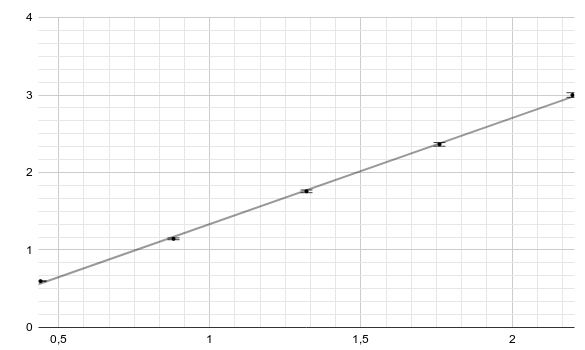
\includegraphics[width=0.9\textwidth]{chart1.png}
    \caption{График зависимости $\ln{\frac{N_0}{N}}$ от толщины поглатителя из свинца}
    \label{fig:my_label}
\end{figure}
Из графика получим, что $\mu = 1.37.$ Тогда используя таблицу, изображенную на рис. 3 получим, что $E_\gamma = 0.6$ МэВ.
\newpage
\item Повторим измерения для железа.

\begin{table}[h]
\caption{Зависимость числа частиц, попадающих на счетчик, от толщины поглотителя из железа}
\resizebox{0.5\textwidth}{!}{%
\begin{tabular}{|l|l|l|l|l|l|}
\hline
\rowcolor[HTML]{FCFF2F} 
  & 1     & 2     & 3     & $\overline{N}$ & $\varepsilon_N$ \\ \hline
1 & 42039 & 42102 & 41377 & 41839          & 1.0\%             \\ \hline
2 & 22428 & 22257 & 22871 & 22518          & 1.4\%             \\ \hline
3 & 12259 & 12135 & 12427 & 12273          & 1.2\%             \\ \hline
4 & 6297  & 6407  & 6587  & 6430           & 2.3\%             \\ \hline
5 & 3247  & 3450  & 3624  & 3440           & 5.9\%             \\ \hline
6 & 1711  & 1687  & 1725  & 1707           & 1.1\%             \\ \hline
7 & 752   & 736   & 772   & 753            & 2.4\%             \\ \hline
\end{tabular}%
}
\end{table}
Учитывая, что толщина одного блока железа равна $1.04$ см, построим график зависимости $\ln{\frac{N_0}{N}}$ от толщины поглатителя из железа. При это мотбросим точку номер $5$ из-за того, что погрешность в ней больше $3\%.$\par
\begin{figure}[h]
    \centering
    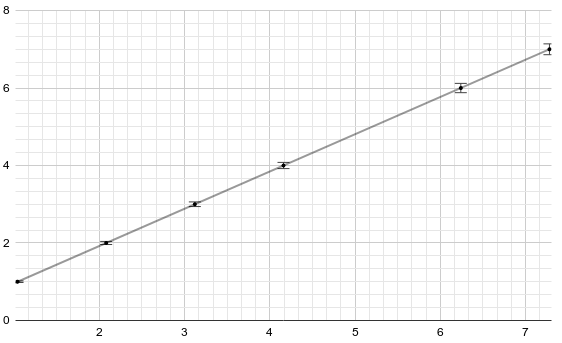
\includegraphics[width=0.9\textwidth]{chart2.png}
    \caption{График зависимости $\ln{\frac{N_0}{N}}$ от толщины поглатителя из железа}
    \label{fig:my_label}
\end{figure}
Из графика получим, что $\mu = 0.96.$ Тогда используя таблицу, изображенную на рис. 3 получим, что $E_\gamma = 0.2$ МэВ.
\newpage
\item Повторим все измерения для алюминия.\par
\begin{table}[h]
\caption{Зависимость числа частиц, попадающих на счетчик, от толщины поглотителя из алюминия}
\resizebox{0.15\textwidth}{!}{%
\begin{tabular}{|l|l|}
\hline
\rowcolor[HTML]{FCFF2F} 
N     & n \\ \hline
49303 & 1 \\ \hline
31464 & 2 \\ \hline
13018 & 4 \\ \hline
8230  & 5 \\ \hline
5341  & 6 \\ \hline
\end{tabular}%
}
\end{table}
Построим график по этим данным, учитывая, что толщина блока алюминия $2.00$ см.\par
\begin{figure}[h]
    \centering
    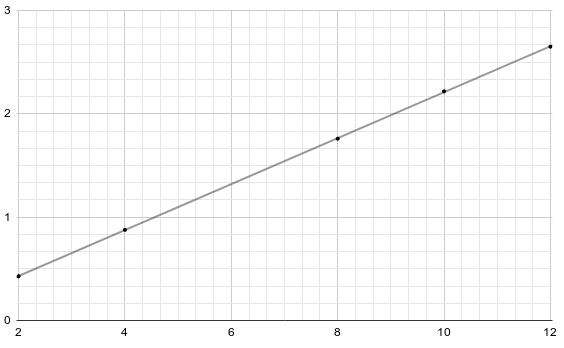
\includegraphics[width=0.9\textwidth]{chart3.png}
    \caption{График зависимости $\ln{\frac{N_0}{N}}$ от толщины поглатителя из алюминия}
    \label{fig:my_label}
\end{figure}
Из графика получим, что $\mu = 0.22.$ Тогда используя таблицу, изображенную на рис. 3 получим, что $E_\gamma = 0.5$ МэВ.
\end{enumerate}

\section{Вывод}
Измеренные по коэффициенту поглощения алюминием и свинцом энергии гамма-квантов оказались близки. Энергия гамма-квантов во всех случаях оказалась слишком мала для того, чтобы образование электрон-позитронных пар вносило существенный вклад. Графики зависимостей получились линейными, что подтверждает теорию о том, что поглощение происходит по экспоненциальному закону.
\end{document}